
\chapter{Lecture}\label{lec16}%% 16 
\setcounter{section}{9}

\subsection{}\label{lec16:sec9:subsec3}

We\pageoriginale continue with the proof of theorem \ref{lec15:sec9:subsec1:thm9.1}. Having proved that
$D_{\tau} u \in H^m (\Omega^\epsilon)$ we proceed to prove now the 
\begin{proposition}\label{lec16:sec9:subsec3:prop9.2} %Proposition 9.2
  $D^p_{\tau} u \in H^m (\Omega^{\epsilon})$ for $|p| \leq m$. 
\end{proposition}

We prove this by induction. Assume it to have been proved for $p = 1,
\ldots$, $r-1$; we prove it for $p=r$. Let $\phi$ be as before in
$\mathscr{D}(\bar{\Omega})$ vanishing near $\partial \Omega-\sum$. To
prove that $D^{\mu}_{\tau} u \in H^m
(\Omega^{\in})$, it is enough to prove that $\phi
D^{\epsilon}_{\tau} u \in H^m (\Omega)$, where $\phi$ is as
in proposition \ref{lec15:sec9:subsec2:prop9.1}. This will follow from the weak compactness
argument used previously if we prove that $(\phi
D^{\mu}_{\tau} u)^{-h} $ is bounded in $H^m (\Omega)$ and this
itself will follow on account of ellipticity if we have proved that  
\begin{equation*}
  |a((\phi D^{\mu}_{\tau} u)^{-h}, v)| \leq c||v||_m \tag{1}.\label{lec16:sec9:subsec3:eq1} 
\end{equation*}

To prove (\ref{lec16:sec9:subsec3:eq1}), we write as before 
\begin{align*}
  a((\phi D u)^{-h}, v)& =(a(\phi D^{\mu}_{\tau} u)^{-h}, v) + a((\phi
  D^{\mu}_{\tau} u), v^h) - a( D^{\mu} u, v^h) -
  b(D^{\mu}_{\tau} u v^{h})\\ 
  \text{where} \hspace{.75cm} b(u, v) & = a(\phi u, v)-a(u \phi v). 
\end{align*}

We prove now in the following three lemmas saying that each of the
terms above is bounded in $H^m(\Omega)$.  

\begin{lemma}\label{lec16:sec9:subsec3:lem9.4} %Lemma9.4
  $\big|a((\phi D^{\mu}_{\tau} u)^{-h}, v)+ a(\phi D^{\mu}_{\tau}
  u^{-h}, v)| \leq c_1||v||_m. $ 
\end{lemma}

\begin{lemma}\label{lec16:sec9:subsec3:lem9.5} %Lemma 9.5
  $\big|a(\phi D^{\mu}_{\tau} u \phi v^h)| \leq c_1 ||v||_m $.
\end{lemma}

\begin{lemma}\label{lec16:sec9:subsec3:lem9.6} %Lemma 9.6
  $\big|b(\phi D^{\mu}_{\tau} u v^{h})\big| \leq c_3 ||v||_m$. 
\end{lemma}

We begin with \ref{lec16:sec9:subsec3:lem9.4}. The expression to be estimated consists of sums
of terms like  
\begin{align*}
  X & = \int (\alpha (x)D^p(\phi D^r_{\tau} u )^{-h} \overline{D^q v}+ (x)
  d^p(\phi D^\mu_{\tau} u )\overline{D^q v^h} dx\\ 
  & = \int ( (\alpha[D^p(\phi D^r_{\tau} u )^{-h} - (\alpha D^p(\phi
    D^r_{\tau} u ))^{-h}] \overline{D^q v} dx \tag*{ by using (\ref{lec16:sec9:subsec3:eq1})} \\
  & = \int \alpha^{-h} D^p \phi D^r_{\tau} u (x-h) \overline{D^q v}
  \tag*{ by using (2)}  
\end{align*}

Since\pageoriginale $|r|= k-1$, by induction hypothesis, $D^r_{\tau} u(x-h)$ is
bounded in $H^{2m}(\Omega^{\in})$ and $\alpha^{-h} D^p ( \phi
D^r_{\tau} u (x-h) \bigg )$ in $L^2$ as $|p| \leq m$, which proves
\ref{lec16:sec9:subsec3:lem9.4}.  

Now we prove \ref{lec16:sec9:subsec3:lem9.5}. We have $a(D^r_{\tau} u \phi v^h) = a(D^r_{\tau}
u \phi v^h) -(-1)^{k-1} a(u\break D^r_{\tau} (\phi u)^h) +$ $ (-1)^{k-1}
a(u, D^r_{\tau} (\phi v)^h)$.  

From 9.2, we have
 $$
 a(u, D^r_{\tau}(\phi v)^h) = (f, D^r_{\tau} (\phi v)^h)_o, \text{ for
 }|r|= k-1 \leq m-1,  
 $$
 and hence $| a(u, D^r_{\tau} (\phi v)^h)|\leq c||v||_m$. 
 
It remains to consider the first difference, which consists of finite
sum of terms  
$$
Z = \int\limits_{|q| \leq m, |p| \leq m, r= k-1} \alpha D^q
    D^r_{\tau} u \overline{D^p \phi v^h} dx- (-1)^{k-1} \int\limits_{
    |q| \leq m, |p| \leq m, |r|= k-1}\alpha D^q D^r_{\tau} u
    \overline{D^p\phi v^h dx} 
$$

By induction hypothesis, if $|q| \leq m-1$, and $|p| \leq m-1, D^p
\phi v^h$ and $D^p( D^r_{\tau} \phi v^{-h})$ are bounded in $L^2$. So
we consider the terms where $|p|=|q| =m$. Now 
$$
\int \alpha D^q u D^p (\overline{D^r_{\tau} \phi v^h}) dx = (-1)^{k-1} \int
D^r_{\tau}(\alpha D^q u) \overline{ D^q \phi v^h}dx 
$$
and terms in $Z$ with $|p| = |q|= m$ become
$$
\sum_{j \geq 1} \int \beta D^{r-j}_{\tau} D^q u \overline{ D^q \phi v^h}dx
$$
which proves that $|Z| \leq c||v||_m$. 

Finally we prove \ref{lec16:sec9:subsec3:lem9.6} $b(D^r u, v^h)$ is a sum of terms like $ \int
\alpha D^q D^r_{\tau} u \overline{D^p \phi v^h} dx$. If $|p| \leq
m- 1$, since $v^h$ are bounded in $H^m, D^p v^h$\pageoriginale are bounded in
$L^2$. If $|p| = m-1$,  
$$
\int \beta D^q D^{r}_{\tau} u \overline{ D^q \phi v^h}dx = - \int (
\beta D^q D^r_{\tau} u )^{-h} \overline{D^p v} dx 
$$
and $v^h$ are bounded in $L^2$. Hence in any case 
$$
|b(D^r_{\tau} u, v^h)| \leq c||v||_m. 
$$

Upto now we followed the proof given by Nirenberg [\ref{k14:e2}]. In the
following, the proof will be slightly more complicated than his, but
will prove slightly more. Another proof is briefly indicated in
Browder \cite{k5}.  

\subsection{}\label{lec16:sec9:subsec4} 

We still require a few preparatory lemmas
before taking up the proof proper of the theorem.  

\begin{lemma}\label{lec16:sec9:subsec4:lem9.7} %Lemma 9.7
  Let $\Omega = ] 0, 1[^n$ be $n$-cube and $u \in L^2 (\Omega)$
      be such that $D^m_i u \in L^2$ where $D^m_i =
      \dfrac{\partial^m}{\partial x^m_i}$(exactly $m$-th derivatives in
      each variable). Then $u \in H^m(\Omega)$.  
\end{lemma}

\begin{remark*}%Remark 
This lemma is related to the theory of \textit{ coercive forms } of
Aronszajn [\ref{k2:e1}].  
\end{remark*}

This lemma will be proved in two steps. 
\begin{enumerate}[(a)]
\item We prove first $D^k_i \in L^2 (\Omega)$for $|k| \leq m-1$. 

  Let $K^m(\Omega)$ be the space of $ u \in L^2$ such that $D^k_i u \in L^2
  (\Omega)$. This is a space of type $H(\Omega, A)$ and hence is a
  Hilbert space with its usual norm. By using Fourier transforms, we see
  that on $\mathscr{D}(\Omega)$ the $K^m$ metric and $H^m$
  metric are equivalent. Hence the closure of $D(\Omega)$ in
  $K^m(\Omega)$ is $H^m_o(\Omega)$. From prop. \ref{lec1:sec1:subsec4:prop1.3}, we have  
  $$
  K^m(\Omega) = H^m_o(\Omega) \oplus \mathscr{H}, 
  $$
  where $f \in \mathscr{H}$ if and only if $\sum (-1)^m D^{2m}_i
  f + f =0$. Now as the operator $\sum (-1)^m D^{2m}_i$ is uniformly
  elliptic, we have $ f \in \mathscr{E} (\Omega)$.  
  
  To\pageoriginale prove (a) we have to prove, say $D^k_1 f(x_1, \ldots , x_n)
  \in L^2 (\Omega), f \in \mathscr{E} (\Omega) \cap
  K^m$. From a classical inequality, we have  
  $$
  \int \limits^{1-\epsilon}_{\epsilon}D^k_1 f(x_1, \ldots ,
  x_n)|dx_1 \leq c\int
  \limits^{1-\epsilon}_{\epsilon}(|f|^2+|D^m_1f|^2)dx_1,  
  $$
  where $c$ is independent of $\in$. Integrating over the
  remaining variables, we have  
  $$
  \int\limits_{\Omega \epsilon}D^k_1 f(x_1, \ldots , x_n)|^2 dx \leq
  c\int \limits_{\Omega \epsilon}(|f|^2+|D^m_1f|^2)dx 
  $$
  for every $\in > 0$. Hence 
  $$
  \int\limits_{\Omega^\epsilon}D^k_1 f(x_1, \ldots , x)|^2 dx \leq c
  ||u||^2_K m \text{ for } f \in \mathscr{H}.  
  $$
  
  We have proved then if $u \in K^m (\Omega)$, then
  $D^k_i u \in L^2$ for all $|k|\leq m-1$.  
  
  \begin{coro*}%Corollary
    If $\mathscr{O} \in \mathscr{D}(\Omega) \text{ and } u
    \in \mathfrak{K}^m, \text{ then } \mathscr{O} u \in
    \mathfrak{K}^m$.  
  \end{coro*}
  
  This follows at once from Leibnitz's formula, and (a). Now the
  second step is to prove 
\item
  Let 
  $$
  \Omega'=
  \begin{cases}
    -1 < x_1 < 1 \\
    0 < x_i < 1
  \end{cases}
  , i=2, \ldots , n.
  $$
  Then for every $u \in K^m (\Omega)$, there exists
  $U \in K^m (\Omega')$  such that $U=u$a. e. on
  $\Omega$. 
  
  Assuming this for a moment, we finish the proof of the lemma, Applying
  $(b)$ to each of variables $x_i$, we get an open cube $Q$ such that
  $\bar{\Omega} \cap Q$ and such that for every $ u \in
  K^m (\Omega)$, there exists $ U \in K^m
  (\Omega)$ with $U=u$ a.e. on $\Omega$. Let $\mathscr{O}$ be a function
  in $\mathscr{D}(Q)$ which is 1 on $\Omega$. Then by the corollary
  to $(a), \theta U \in K^m (Q)$ and having compact
  support is in $H^m_o (\Omega)$. Hence its restriction to $\Omega$
  which is $u$ is in $H^m(\Omega)$.  

  Now to prove $(b)$, we require 
\item $\mathscr{D}(\bar{\Omega})$ is dense in $K^m (\Omega)$. 
  
  We may obviously assume $\Omega=]-1, 1[^n \cdot$. Let $u \in
      K^m (\Omega)$ and define $v_t(x) = v(tx)$, for $t< 1$ for all $x
      \in \Omega$ such that $x \in \dfrac{1}{t} \Omega$.  
\end{enumerate}

Let\pageoriginale $u_t$ be the restriction of $v_t$ to $\Omega$. Then it is
easily seen that as $t \to 1, u_t (x) \to u(s)$ in $K^m
(\Omega)$. Hence to prove $(c)$ it is enough to prove that each
$u_t (x)$ can be approached by functions of $\mathscr{D}
(\bar{\Omega })$. Since $\bar{\Omega} \subset \Omega '$, let $\theta$
be a function in $\mathscr{D} (\bar{\Omega})$ which is $1$ on
$\bar{\Omega}$. Then $\omega = \theta v_\tau (x) K^m
(\Omega')$ and has compact support. Hence $\omega \in H_0^m
(\Omega ')$ and so $\omega = \lim \varphi_k$ in $H_o^m (\Omega ')$
where $\varphi_k \in \mathscr{D} (\Omega ')$. Hence
restrictions of $\varphi_k $ to $\Omega$ converge to $u_\tau = $
restriction of $\omega$ to $\Omega$ in $K^m (\Omega)$.  

Now we prove $(b)$. It is enough to define a map from
$\mathscr{D}(\bar{\Omega})$ to $K^m (\Omega')$ which is
continuous in $\mathscr{D} (\bar{\Omega })$ with the topology of
$K^m (\Omega)$. Let $u(x) \in \mathscr{D}
(\bar{\Omega})$ and let $\Omega '$ be as in $(b)$. Define 
$$
U(x) = 
\begin{cases}
  u(x) \text{ in } \Omega . \\
  \lambda_1 u(x', -x_n) + \cdots + \lambda_n u(x ' - \frac{x_n}{n})
\end{cases}
$$
where $x' = (x_1, \ldots , x_{n-1})$ and $(x', x_n) \in \Omega
' - \Omega$. We find $\lambda_i$ suitably so that all the Derivatives
of $U$ on $\Sigma$ are well defined. (See \S\ \ref{lec4:sec2:subsec5}). This mapping $u
\to U $ of $\mathscr{E} (\Omega)$ with the topology of $K^m
(\Omega)$ to $K^m (\Omega ')$ is seen at once to be
continuous. This finishes the poof of lemma \ref{lec16:sec9:subsec4:lem9.7}.  
\begin{figure}[H]
  \centering{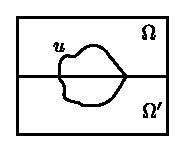
\includegraphics{vol10-figures/fig10-chap16-1.eps}}
\end{figure}
